\chapter{Model Order Estimation}
\label{ch:ModelOrderEstimation}

\section{Introduction}
Model selection is a broad field in statistical analysis and signal processing, focusing on selecting the optimal model
from a set of candidate models based on specific criteria or metrics~\cite{costa2009}.
Within this context, \glsdesc{moe}%
\footnote{%
    Also referred to as \textit{model order selection} in the literature.
}
seeks to ascertain the most suitable number of parameters or components for fitting a model to a given dataset~\cite{barthelme2020}.\\
Classical methods for \gls{moe}, known as \glspl{ic}, aim to balance the goodness of fit of a model to the data
adversarial to its complexity by employing some form of regularization to avoid overfitting.

\subsubsection*{MOE in the Field of DOA Estimation}
In the domain of \gls{ddf}, \gls{moe} is concerned with discerning the count of incident far-field wave-fronts,
simultaneously impinging on an antenna array like a \gls{uca}.
The estimation of the model order is a crucial step in \gls{doa} estimation, as it fundamentally allows the selection
of the most likely signal model among several candidates~\cite{barthelme2020}.\\
As outlined in Section~\ref{sec:sub:subspaces}, the model order \( N \) corresponds to the rank of the signal subspace
\( \bfm{U}_S \) and also equals the number eigenvalues that are different from the smallest eigenvalue.
This assumption holds when all \( N \) incoming signals are uncorrelated and thus linearly independent and \( \C \rightarrow \bfm{C}_x \),
which can be assumed to be true for \( K \gg M \)~\cite{trees.ch7}.\\
As mentioned earlier, super-resolution algorithms such as \gls{music}, elaborated upon in the previous
chapter, rely on an accurate estimate of the model order \( \NPred \) for effective subspace decomposition (\( \bfm{U} = \bfm{U}_S \oplus \bfm{U}_N \)).
Furthermore, the operator of a \gls{ddf} system or a sophisticated policy-selection algorithm might use the condition
\( \NPred \overset{?}{>} 1 \) as a criterion to select the most suitable direction finding algorithm.


\section{Classical Information Criteria}
\label{sec:ClassicalInformationCriteria}
The \gls{aic} and the \gls{mdl}, both classical \glspl{ic},
are frequently employed for \gls{moe}. They were first utilized to determine the number of impinging wavefronts by introducing
a convenient reparametrization of the maximum likelihood estimate of the underlying signal model in~\cite{mdlAndAic}.
The general form of the log-likelihood function for our data model is given by:

\begin{equation}
    \NPred=\underset{n \in \NSet}{\argmax} \ln \left(p_{n}\left(\bfm{x} ; \widehat{\bfT}, \C, \widehat{\sigma}_\eta^2\right)\right)+ c(n)
    \label{eq:max_likelihood}
\end{equation}

The maximum likelihood estimate is denoted by \( p_{n}(\cdot) \), and \( c(n) \) is a regularization term that penalizes
large model orders~\cite{barthelme21sub}.
The reparametrization of the likelihood estimate significantly increases the simplicity of the
model order estimation problem, as it allows the likelihood function to be solely expressed in terms of the eigenvalues of the
covariance matrix \( \C \).
The essence of these classical approaches to \gls{moe} lies in discerning the set of eigenvalues from a covariance matrix that significantly diverge
from a tightly grouped cluster with low variance, which is centered around the noise variance \( \sigma^2_{\eta} \).
The aim is to reduce the variance among the smallest \( M - n \) eigenvalues, while adversarially penalizing large
values for \( M - n \) to avoid overfitting.\\


Central to both criteria is the ratio between the arithmetic mean \( \am(\bfL_n) \) and the geometric mean
\( \gm(\bfL_n) \) of the \( M - n \) smallest eigenvalues.\\
It is expressed as:
\begin{equation}
    \am(\bfL_n) \coloneqq \frac{1}{M-n} \sum_{i=n+1}^{M} \lambda_i
\end{equation}

Similarly, the geometric mean for these eigenvalues is:
\begin{equation}
    \gm(\bfL_n) \coloneqq \sqrt[M-n]{\prod_{i=n+1}^{M} \lambda_i}
\end{equation} %TODO: starting idx??

The ratio of the geometric mean to the arithmetic mean equals one when all eigenvalues are identical, reflecting a
uniform distribution—this would be the case for an ideally estimated subspace of \gls{awgn}.
A higher ratio indicates a departure from a uniform distribution in the set of considered eigenvalues, thus highlighting
the presence of signal eigenvalues. Both \glspl{ic} exploit this relationship, seeking the subset of
eigenvalues that most closely mirror a uniform distribution, and thereby distinguishing the noise subspace
from the signal subspace \( \bfm{U} = \bfm{U}_S \oplus \bfm{U}_N \)~\cite{meyer}.\\
For ease of reference and clarity, we define \( \NSet \) as the set of potential model orders. Specifically,
\( \NSet \coloneqq \{1, \ldots, N_{\max}\} \), where \( N_{\max} = M - 1\) is the maximum possible number of incoming signals%
\footnote{
In practice, \( N_{\max} \) is often set to a lower value to simplify computations, since the likelihood of encountering
up to \( M - 1 \) incoming signals is often negligible.
}.\\

\subsubsection{Akaike Information Criterion (AIC)}

For each potential model order \(n \in \NSet \), the AIC criterion \( \bfm{\mathrm{AIC}} \) can be represented as~\cite{mdlAndAic}:
\begin{equation}
    \bfm{\mathrm{AIC}}[n] = - 2 \cdot \underbrace{{\ln \left(\frac{\gm(\bfL_n)}{\am(\bfL_n)}\right)}^{K(M - n)}}_{log-likelihood} + \underbrace{2n(2M - n)}_{\text {regularization term }} \quad \text{for each } n \in \NSet
    \label{eq:AIC}
\end{equation}


Employing our previous notations, \( M \) denotes the number of antennas and \( K \) the snapshot count.
The estimated model order \( \NPred_\mathrm{AIC} \) can then be calculated as:

\begin{equation}
    \NPred_\mathrm{AIC}=\underset{n \in \NSet}{\argmin}\{ \bfm{\mathrm{AIC}}[n] \}
    \label{eq:AIC_argmin}
\end{equation}

\subsubsection{Minimum Description Length (MDL)}
The MDL criterion is formulated as~\cite{mdlAndAic}:
\begin{equation}
    \bfm{\mathrm{MDL}}[n]=  - {\ln \left(\frac{\gm(\bfL_n)}{\am(\bfL_n)}\right)}^{K(M - n)} + \frac{1}{2} n(2 M-n) \ln (K)
    \label{eq:MDL}
\end{equation}

The estimated model \( \NPred_\mathrm{MDL} \) order can than be calculated in the same fashion as in \autoref{eq:AIC_argmin}.\\
Both \gls{aic} and \gls{mdl} are based on the same principle, but differ in their approach to penalizing large model orders.
While both criteria linearly penalize the model order \( n \), \gls{mdl} additionally tends to favor smaller model orders given
an increasing number of snapshots.
\gls{mdl} tends to yield a more consistent model order estimate than \gls{aic}, which is more prone to overfitting in non-subsampled
scenarios~\cite{mdlAndAic, barthelme2020}.\\


\subsubsection{A Practical Example of Model Order Estimation}
\autoref{fig:aic_mdl_criteria} illustrates the application of \gls{aic} and \gls{mdl} to predict the model order for
a scenario, drawn from the dataset \( \DMain_{(\text{test})} \), with \( M = 9 \) antennas and \( K = 100 \) snapshots
and the use of the incoherent covariance matrix \( \Csub \).

\begin{figure}[H]
    \centering
    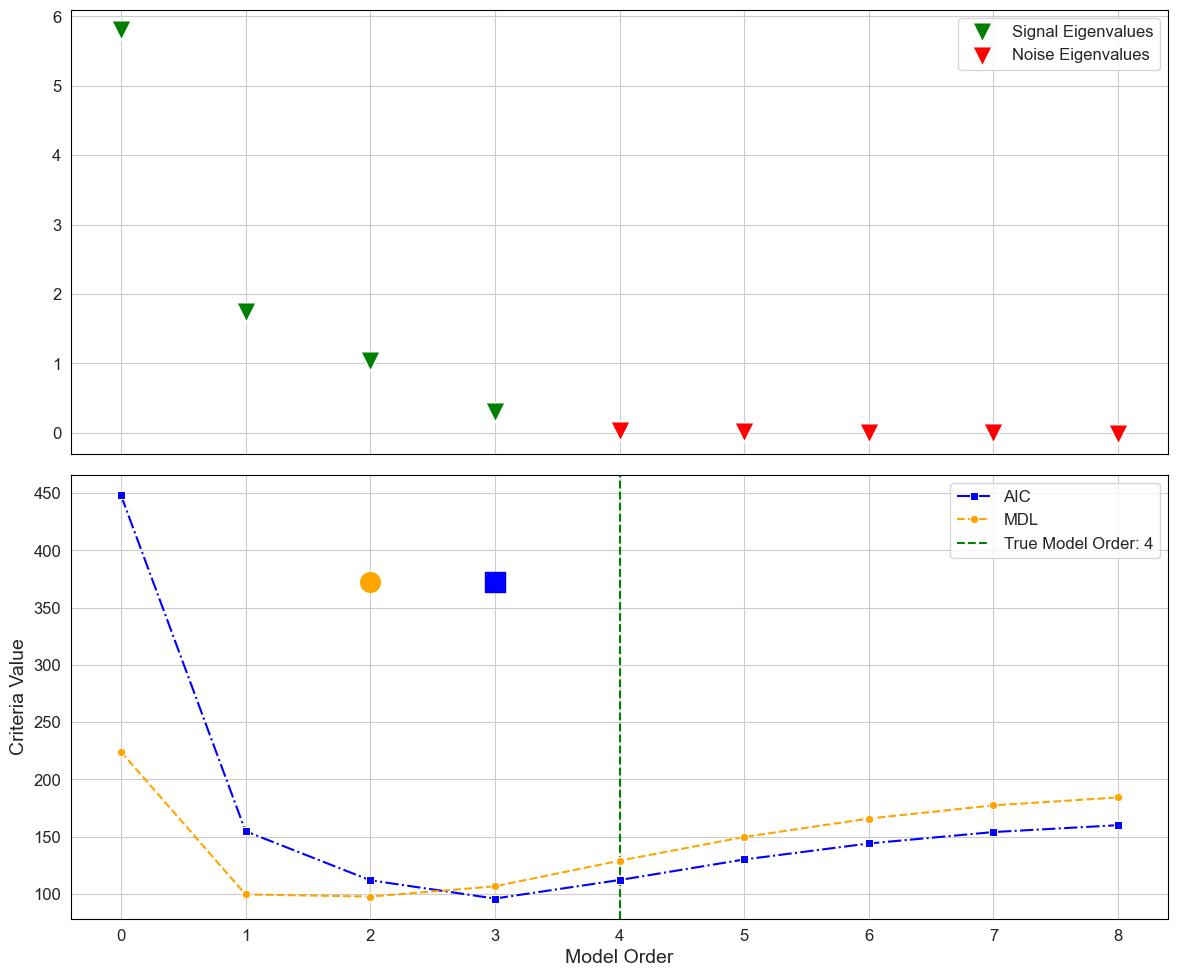
\includegraphics[width=0.8\textwidth]{figures/04_ModelOrderEstimation/aic_mdl_criteria.png}
    \caption{A working example of the \gls{aic} and \gls{mdl} estimators.}
    \label{fig:aic_mdl_criteria}
\end{figure}

For this setup, the \gls{aic} predicted a model order \( \NPred_\mathrm{AIC} = 3 \), while \gls{mdl} estimated
\( \NPred_\mathrm{MDL} = 2 \), reflecting the impact of the more pronounced regularization term in \gls{mdl}.
The underfitting of the model order prediction is not expected, given the actual \gls{snr} and \gls{sir} values, with \( \mathrm{SIR}_{\max} = 10.86 \, \text{dB} \)
and \( \mathrm{SNR}_{\min} = 14.77 \, \text{dB} \). \\
The reason for the underwhelming performance of the \gls{aic} and \gls{mdl} criteria in this
scenario is due to effects of sub-sampling and the ``limited'' number of snapshots \( K \).
The former effect seems to be the primary reason for a pronounced bias towards underestimating the model order.
These repercussions will be the subject of further investigation in \autoref{sec:challenges_moe} and \autoref{ch:evaluation_results}.



\section{Exponential Fitting Test (EFT)}
\label{sec:eft}
\subsection{Introduction}
The \glsdesc{eft}, first introduced by~\cite{eft} in 2007, marks an algorithmical paradigm shift the domain of \gls{moe}
the \gls{eft} aims to directly detect gap a gap between the noise and signal eigenvalues, rather than relying on
the indirect approach of discerning a uniform distribution among the noise eigenvalues.
It was designed to overcome the limitations of traditional methods when dealing with non-coherent sources and a small
number of snapshots, all while maintaining computational complexity comparable to the \glspl{ic} discussed in \autoref{sec:ClassicalInformationCriteria}.
The \gls{eft} leverages the observation that the descendingly ordered noise eigenvalues approximately exhibit exponential decay.
The algorithm seeks to robustly predict the model order by identifying discrepancies
that exceed a predetermined threshold between the observed eigenvalues and the
anticipated exponential decay curve, thereby effectively distinguishing between signal and noise. \\

Despite subsequent enhancements to the \gls{eft} as detailed in~\cite{costa2007} and~\cite{costa2009}, the original version
has been implemented as a baseline for comparative analysis against classical methods like \gls{aic} and \gls{mdl} and
the \glspl{dnn} architectures explored in this thesis.\\

\subsection{Algorithm}
\subsubsection*{Estimating the Decay Coefficients}

The \gls{eft} algorithm employs a recursive approach to model the exponential decay pattern of noise eigenvalues.
This decay is represented by\footnote{To distinguish between the predicted and observed eigenvalues, of the
\textit{estimated} covariance matrix \( \C \), the former are denoted as \( \hat{\lambda} \), while the estimated
observed eigenvalues will be denoted without their hat \( \widehat{\bullet} \).}:
\begin{equation}
    \hat{\lambda}_i = \lambda_1 \cdot {q(M, K)}^{i-1} \quad \text{for } i \in \NSet, \; q \in (0, 1)
    \label{eq:eft_decay_coeff}
\end{equation}
In \autoref{eq:eft_decay_coeff}, \( \lambda_1 \) represents the largest eigenvalue in a noise-only scenario, and \( q(M, K) \) is the decay
coefficient, which varies based on the number of antennas \( M \) and the number of snapshots \( K \).
The challenge lies in accurately determining the decay coefficient \( q : (M, K) \rightarrow \mathbb{R} \) to estimate
exponential decay of the noise eigenvalues.

\cite{eft} derived a method to estimate \( q \) based on the first order approximation of the noise variance \( \sigma^2_{\eta} \)
aussiming a noise-only scenario:
\begin{equation}
    \sigma^2_{\eta} \approx \frac{1}{M} \sum_{i=1}^{M} \lambda_i
    \label{eq:eft_noise_variance}
\end{equation}

Through a series of mathematical transformations, detailed in~\cite{eft}, a relation involving \( q \) is formulated:
\begin{equation}
    \frac{M+K}{M K} = \frac{(1-q)\left(1+q^M\right)}{\left(1-q^M\right)(1+q)}
\end{equation}

Solving this equation for \( q \) involves using a substitution \( q = \exp(-2a) \) and subsequently solving the
resultant cubic equation for \( a \):
\begin{equation}
    a=\sqrt{\frac{1}{2}\left\{\frac{15}{M^2+2}-\sqrt{\frac{225}{\left(M^2+2\right)^2}-\frac{180 M}{K\left(M^2-1\right)\left(M^2+2\right)}}\right\}} .
    \label{eq:eft_decay_coefficient}
\end{equation}

\subsubsection*{Iterative Eigenvalue Prediction and Comparison}
Following the calculation of the pre-computable decay coefficient \( q \), the predictive process of the \gls{eft} algorithm
begins by assuming the smallest observed eigenvalue \( \lambda_M \) to be part of the noise subspace,
setting the initial noise subspace dimension \(  p= 1 \). The process iteratively predicts each subsequent
eigenvalue according to the assumed exponential decay pattern, expanding the candidate noise subspace and recalculating
\( \hat{\lambda}_{M-p} \) from the updated estimate of the noise variance \( \widehat{\sigma}^2_{\eta} \).
This evaluation continues until a significant mismatch between the observed eigenvalue and the predicted noise profile is detected.
The predicted eigenvalue \( \hat{\lambda}_{M-p} \) is calculated as:
\begin{equation}
    \hat{\lambda}_{M-p} = \frac{1 - q(M, K)}{1 - {q(M, K)}^{p + 1}} \cdot \underbrace{\sum_{i=0}^{p}\lambda_{M-i}}_{(p+1)\widehat{\sigma}^2\eta}
    \label{eq:eft_predicted_eigenvalue}
\end{equation}


\subsubsection*{Hypothesis Testing}

With each iterative step of the \gls{eft} process, two competing hypotheses are considered for the eigenvalues under
examination:

\begin{align}
    \mathcal{H}_{p+1} &: \lambda_{M-p} \in \bfL_\eta \label{eq:hypothesis_noise} \\
    \widetilde{\mathcal{H}}_{p+1} &: \lambda_{M-p} \in \bfL_S \label{eq:hypothesis_signal}
\end{align}

Starting with the pair \( (\lambda_{M-1}, \hat{\lambda}_{M-1}) \), the relative distance between each of the
theoretical noise eigenvalues and their corresponding observed eigenvalue is computed. This difference is then assessed
against a predefined threshold value \( \tau_n \), which scales with the eigenvalue index. The condition for
determining the hypothesis to accept is as follows:

\begin{equation}
    \text{accept } \left\{
        \begin{array}{ll}
            \mathcal{H}_{p+1}, & \text{if } \left|\frac{\lambda_{M-p} - \hat{\lambda}_{M-p}}{\hat{\lambda}_{M-p}}\right| = \epsilon_n \leq \tau_n, \\
            \widetilde{\mathcal{H}}_{p+1}, & \text{otherwise}.
        \end{array}
    \right.
    \label{eq:threshold_condition}
\end{equation}


If the relative difference falls within the threshold, the eigenvalue is classified as noise; otherwise, it is considered
to be an eigenvalue of the signal subspace.
The process iterates, comparing each predicted noise eigenvalue with its observed counterpart,
until a relative error \( |\epsilon| > \tau \) is encountered, signifying a departure from the noise eigenvalue pattern and the
detection of the smallest signal eigenvalue.\\
\autoref{eq:threshold_condition} as proposed in \cite{eft} could classify a \( (\lambda_n, \hat{\lambda}_n) \) pair
as signal if the predicted eigenvalue is smaller than its observed counterpart, which seems unsound. Thus, the signed
relative error \( \epsilon \) should be used instead of the absolute relative error \( |\epsilon| \) in \autoref{eq:threshold_condition}.
The estimated dimension of the noise subspace \( \widehat{p} \) is thus determined to be the value
of \( p \) at which the hypothesis \( \mathcal{H}_{p+1} \) is rejected in favor of \( \widetilde{\mathcal{H}}_{p+1} \). Consequently, the estimated
model order, is given by \( \NPred = M - \widehat{p} \), marking the completion of the \gls{eft} process.\\

\begin{figure}[H]
    \centering
    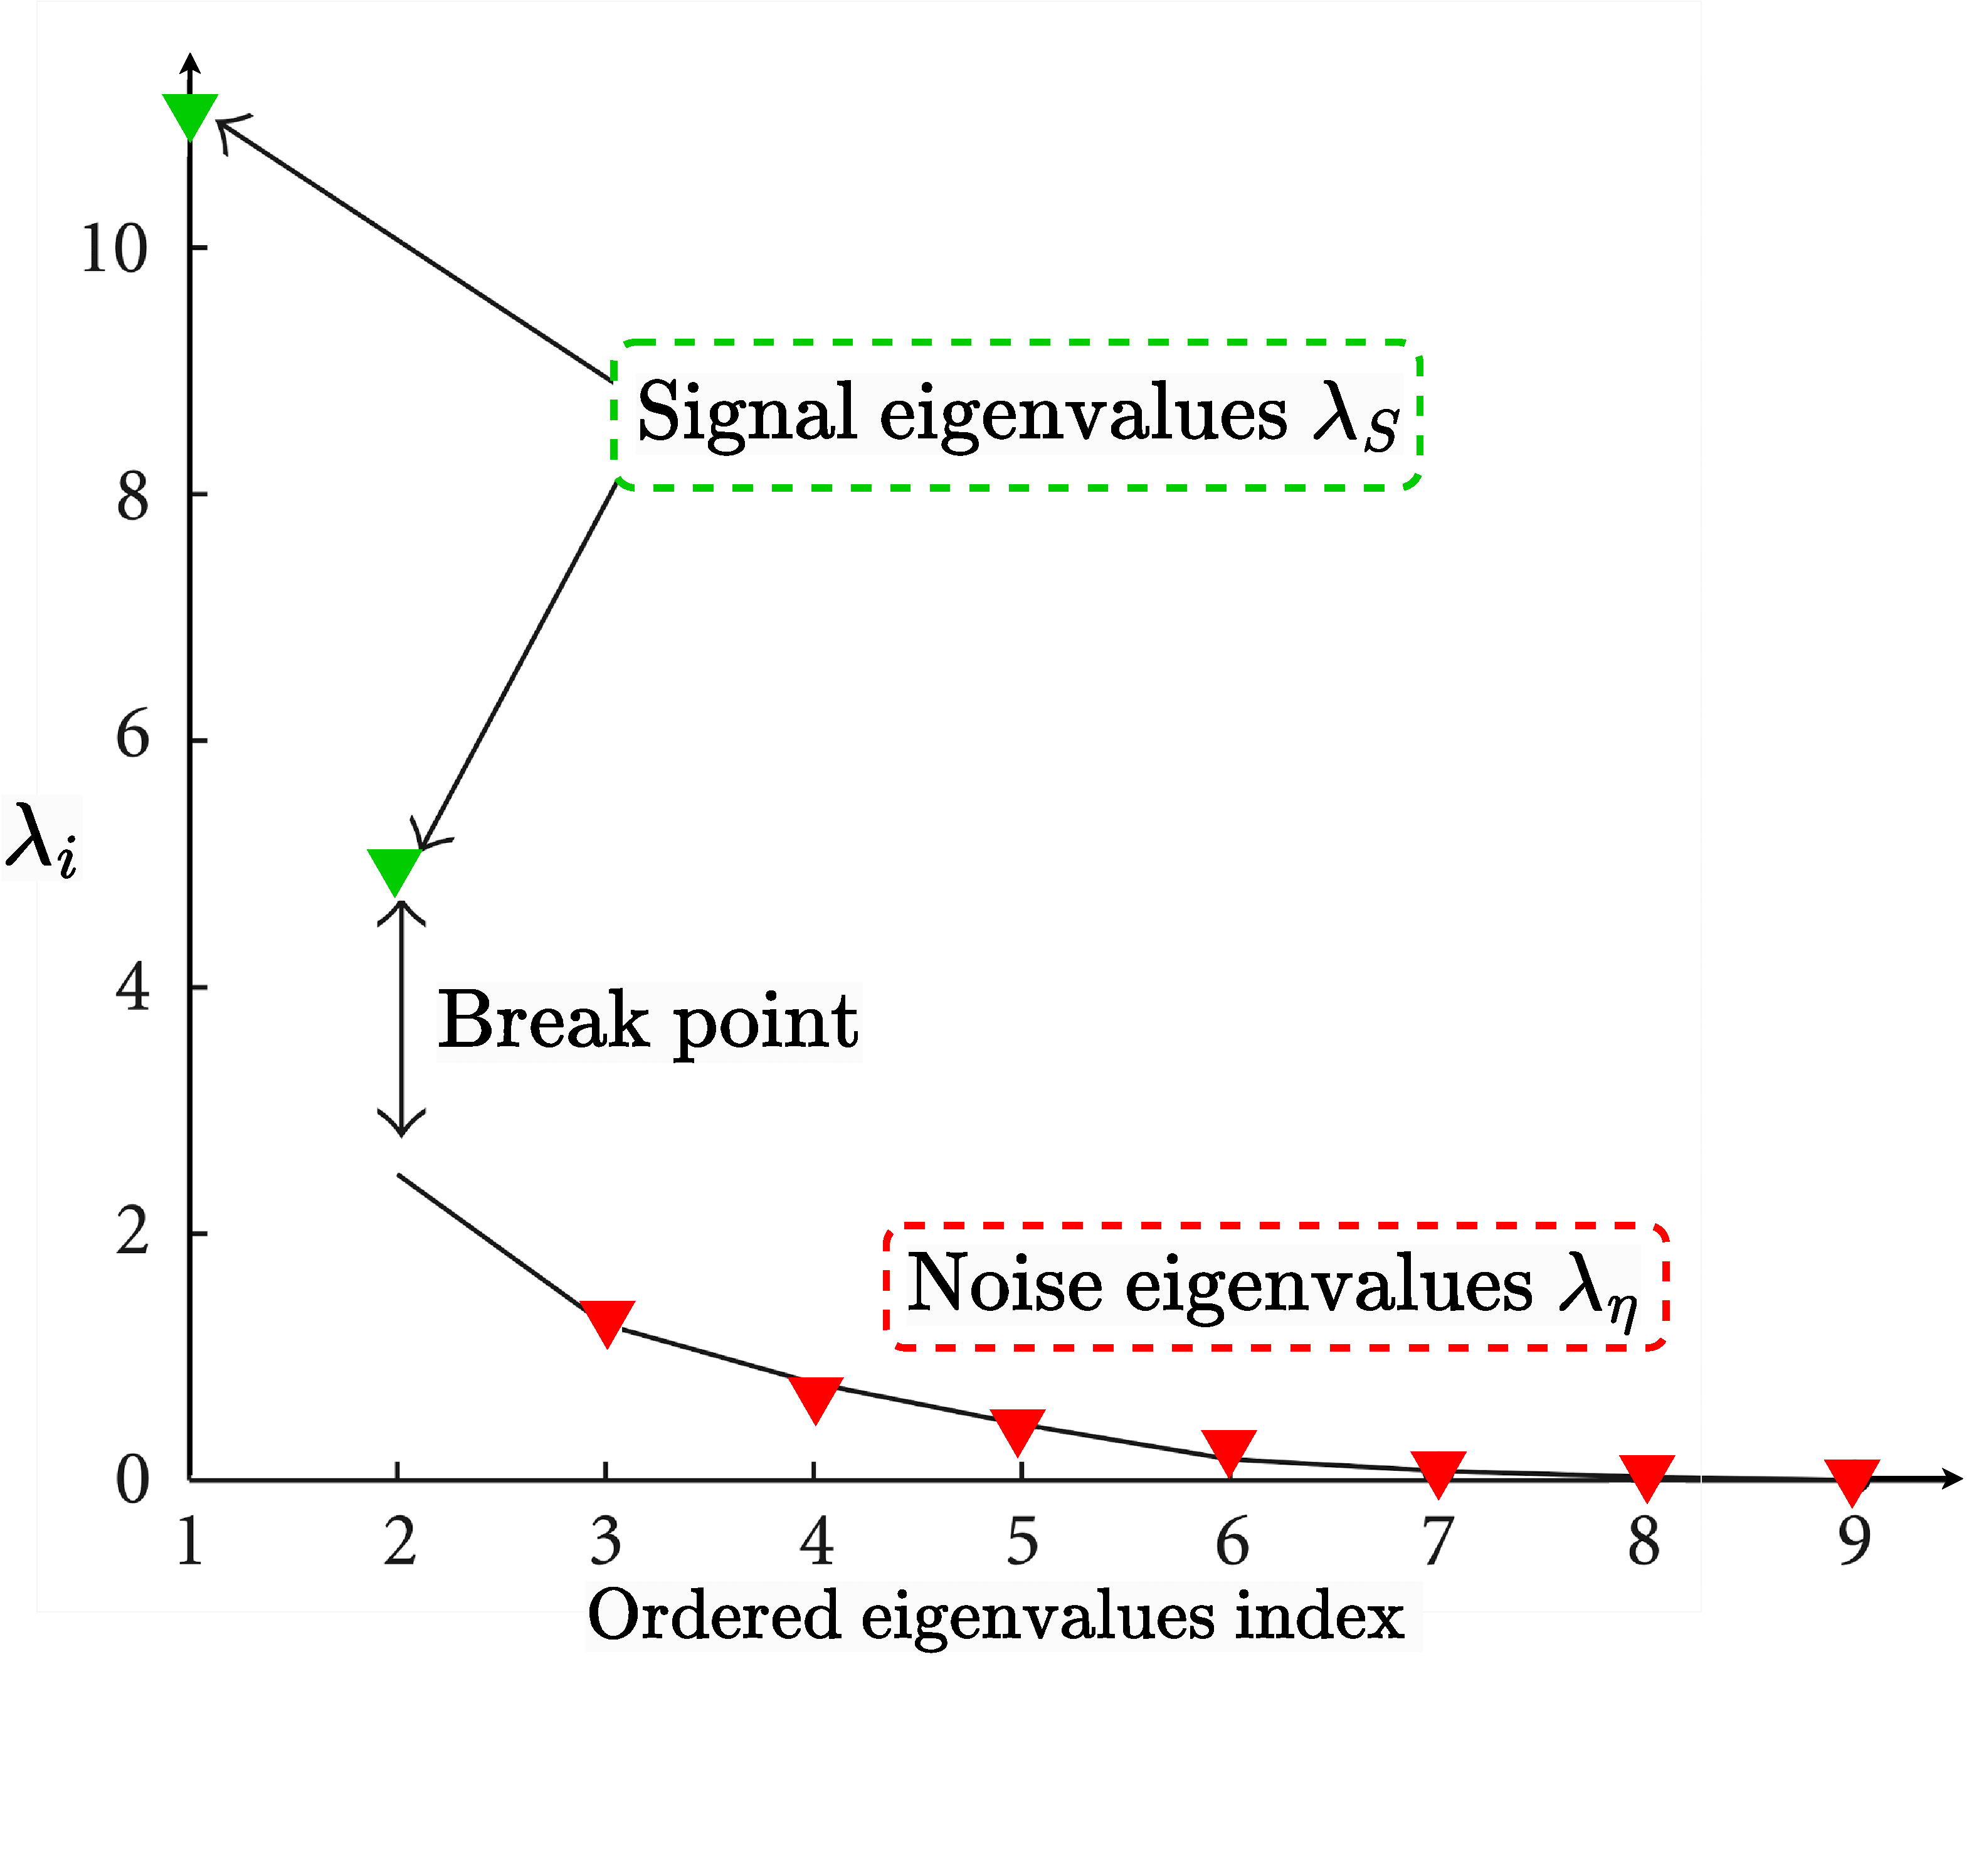
\includegraphics[width=0.55\textwidth]{figures/04_ModelOrderEstimation/eft_scheme.pdf}
    \caption{Conceptual illustration of the \gls{eft} technique-adapted from~\cite{eft}.}
    \label{fig:eft_scheme}
\end{figure}

\autoref{fig:eft_scheme} illustrates the \gls{eft} process for a scenario with \( M = 9 \) antennas and a model order of
\( N = 2 \). The eigenvalue distribution in the figure exposed the discrepancy between the noise and signal
eigenvalues.
For a given \( p = 7\), the hypothesis \( H_{7 + 1} \) is rejected in favor of \( \widetilde{H}_{7 + 1} \), revealing
the smallest signal eigenvalue to have the index \( M - \widehat{p} = \NPred = 2 \). This corresponds to the actual model order.


\subsection{Threshold Calculation}
Similar to the approach in the original study~\cite{eft}, the threshold values \( \epsilon_n \) were calculated based on
predefined false positive rates \( \bfm{F} \) for each possible model order \( n \in \NSet \).
The original study employed a single false positive rate of \( 1 \% \). However, this may not be optimal as eigenvalues
with higher indices are more likely to be checked, increasing the likelihood of false positives for these indices due to
the increased check frequency.

\begin{algorithm}[H]
\label{alg:eft_threshold_calculation}
\caption{EFT Threshold Calculation}
\DontPrintSemicolon
\KwIn{\;
\quad \( \bfm{E} \): Relative errors, calculated as per \autoref{eq:threshold_condition} on the train set\;
\quad \(\bfm{F}\): List of desired false positive rates for each potential signal eigenvalue\;
\quad \(N_{\max}\): Max model order}
\KwOut{\;
\quad \(\bfm{\tau}\): List of threshold values}

\SetKwFunction{FMain}{CalculateEFTThresholds}
\SetKwProg{Fn}{Function}{:}{}
\Fn{\FMain{\(\bfm{E}\), \(\bfm{F}\), \(N_{\max}\)}}{
    \(\bfm{\tau} \gets\) empty list\;
    \For{\(i \gets 0\) \KwTo \(N_{\max}\)}{
        \(\bfm{S} \gets \bfm{E}\) where \( N \leq i\)\;
        \(\bfm{S}_{\text{sorted}} \gets\) sort(\(\bfm{S}[:, i]\))\;
        \(L \gets\) length(\(\bfm{S}_{\text{sorted}}\))\;
        \(\mathrm{Idx} \gets \min(\left\lfloor(1 - \bfm{F}[i]) \cdot L\right\rfloor, L - 1)\)\;
        \(\tau_i \gets \bfm{S}_{\text{sorted}}[\mathrm{Idx}]\)\;
        Append \(\tau_i\) to \(\bfm{\tau}\)\;
    }
    \KwRet \(\bfm{\tau}\)\;
}
\end{algorithm}

Utilizing algorithm \autoref{alg:eft_threshold_calculation}, the following treshold values \( \bfm{\tau} \) were calculated
for the the respective false positive rate

\begin{table}[h]
    \centering
    \caption{Calculated EFT tresholds}
    \begin{tabular}{ccc}
    \toprule
    \( n \:/\: \NPred \) & FPR & \( \tau \) \\
    \midrule
    0 & 0.1 & 0.021 \\
    1 & 0.084 & 0.485 \\
    2 & 0.064 & 0.591 \\
    3 & 0.048 & 0.716 \\
    4 & 0.048 & 0.836 \\
    5 & 0.048 & 0.981 \\
    \bottomrule
    \end{tabular}
    \label{tab:eft_thresholds}
\end{table}

\subsubsection*{Conclusion}

\textbf{Threshold Adjustment and Bias Control:} The EFT aims for a delicate balance between the false
positive rate and the false negative rate, by accordingly adjusting the threshold values \( \tau_n \) for each potential
signal eigenvalue. This enables the EFT to explicitly control potential biases for over- or underestimation.
This balance is inherently tied to the careful selection and optimization of the threshold values
\( (\tau_1, \ldots, \tau_{M-1}) \), which introduce a degree of subjectivity but also a potentially
unwanted dependence that is not present in the parameter-free methods \glspl{ic}.\\
The procedure of selecting the threshold values should be invesiagted further. The following approaches could be considered:
\begin{itemize}
    \item Introduce an optimization process that considers the false negative rate in addition to the false positive rate.
    \item Investigate the choices of different false positive rates to compensate for the increased checking frequencies of
    eigenvalues with higher indices.
    \item After indentifying a suitable set of threshold values, utilize an objective driven optimization process to finetune
    the values. Empirical evidence which was gathered during the optimization of a single threshold value, indicates that
    the optimization problem is at least partially convex. Rather than optimizing all treshold values simultaneously,
    the optimization could be performed sequentially, starting with the threshold value for the smallest potential signal
    eigenvalue.~\autoref{fig:eft_treshold_optim} depicts the plot of the optimization process for a single threshold value.
\end{itemize}
%TODO Adapt plot!
\begin{figure}[H]
    \centering
    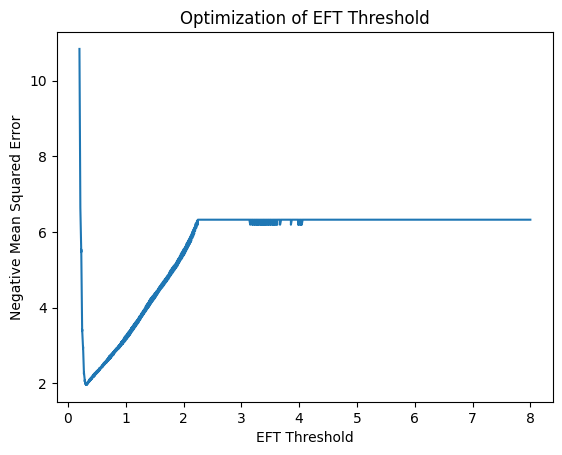
\includegraphics[width=0.5\textwidth]{figures/04_ModelOrderEstimation/eft_treshold.png}
    \caption{Optimization of a single EFT threshold value, where all \( \tau_n \) in \( \bfm{\tau} = \tau \)}
    \label{fig:eft_treshold_optim}
\end{figure}
The tresholds in \autoref{tab:eft_thresholds} differ significantly from the values which were identified in~\cite{eft}.
For \( N_{\max} = 4 \), the original study identified the following threshold values:
\[
    \bfm{\tau} = \left[26.34, 3.647, 1.238, 0.6336 \right]
\]
The divergence between the two sets of threshold values has not been subject to further scrutiny, as the EFT estimators
demonstrated superior performance compared to the AIC and MDL estimators.\\
Additionally, the transferability of these optimized threshold values to different scenarios has yet to be ascertained.
It has been observed that the EFT, with thresholds tailored to a dataset featuring a static snapshot count \( K = 100 \),
exhibited superior performance over the AIC and MDL when applied to a dataset with a variable snapshot count \( K \in [1, 1000] \).
Further details on this comparison are presented in \autoref{sec:influence_num_snapshots}.\\

\textbf{Computational Complexity:} As per~\cite{eft}, the computational complexity of the EFT is on par with that of AIC
and MDL. This assertion is presumably based on the shared requirement of these methods for an eigenvalue decomposition of
the covariance matrix. However, the EFT necessitates considerably fewer computations for the predictive steps, which are
contingent on the eigenvalues. The only computations required at runtime are:

\begin{itemize}
    \item In Equation \ref{eq:eft_predicted_eigenvalue}, the computation involves the summation of the assumed noise
    eigenvalues \( \bfL_\eta \), followed by a multiplication with the precomputed fraction for each potential model order.
    \item In Equation \ref{eq:threshold_condition}, the computation involves \( N_{\max} \) divisions and comparisons.
\end{itemize}

This computational requirement is significantly less than that of the AIC and MDL criteria, which necessitate the
computation of the logarithm of the geometric and arithmetic mean of the eigenvalues, in addition to subsequent
exponentiation for each potential model order.

\textbf{Specific Design for Incoherent Sources:} Tailored to perform well in the presence of incoherent sources,
the EFT's efficacy in environments with coherent sources or multipath interference has not been evaluated.

\textbf{Implementation Caution:}
The Python implementation of the EFT for this thesis presents some inconsistencies when compared to the original EFT
algorithm. A particular point of ambiguity is the calculation of the decay coefficient \( q \), which is not clearly
defined in the original study as to whether it depends on the number of snapshots \( K \) and the noise subspace
dimension \( p \), or on the number of snapshots \( K \) and the number of antennas \( M \).
The notation \( q : (p + 1, K) \rightarrow \mathbb{R} \) versus \( q : (M, K) \rightarrow \mathbb{R} \) is used in~\cite{eft}'s
equivalent to \autoref{eq:eft_predicted_eigenvalue} and is the source of this uncertainty.\\
Both possible versions have
been implemented, but the version with \( q(p+1, N) \) tends to result in estimated exponential decay profiles which
exhibit an unexpected curvature for an exponential function, as depicted in \autoref{fig:eft_coeff_comparison}.
Therefore the version with \( q(M, N) \) is used in this thesis.\\
Another point of ambiguity is the estimation of the noise variance \( \widehat{\sigma}^2_{\eta} \) in \autoref{eq:eft_predicted_eigenvalue}.
According to~\cite{eft}, the noise variance is estimated as the arithmetic mean of the \( p + 1 \) smallest eigenvalues,
this means that \( \lambda_n \) is utilized in the estimation of the noise variance, which will then be used to calculate
\( \hat{\lambda}_n \). This might introduce a bias towards underestimating the model order.

\begin{figure}[H]
    \centering
    \subfloat[]{{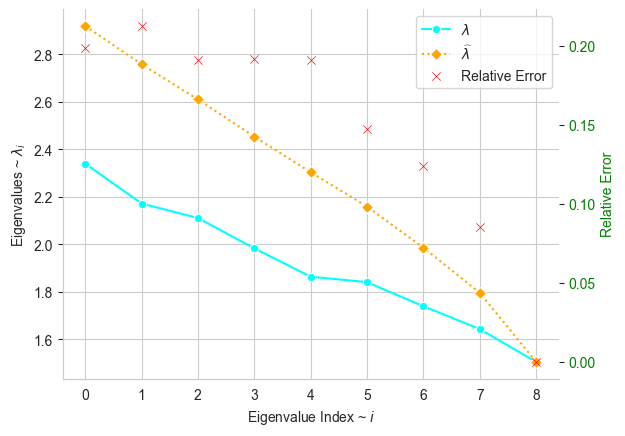
\includegraphics[width=0.45\textwidth]{figures/04_ModelOrderEstimation/eft_wrong_coeff.png}}}
    \subfloat[]{{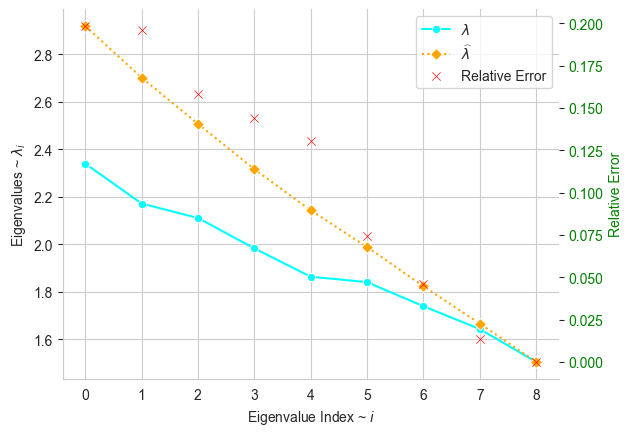
\includegraphics[width=0.45\textwidth]{figures/04_ModelOrderEstimation/eft_correct_coeff.png}}}
    \caption{Comparison of the EFT's predicted eigenvalues, with the decay coefficient \( q \) calculated with \( q(p+1, N) \) (a) and \( q(M, N) \) (b).}
    \label{fig:eft_coeff_comparison}
\end{figure}

\newpage{}
\section{Challenges of Eigenvalue Based MOE}
\label{sec:challenges_moe}

\subsection{Degradation of the Eigenstructure through Sub-Sampling}

The application of classical \glspl{ic} such as \gls{aic} and \gls{mdl} for model order estimation critically depends on the
soundness of the re-parameterization of the maximum likelihood function introduced in~\autoref{eq:max_likelihood}.
While robust and effective for coherently sampled covariance matrices, this methodology loses its validity
due to the severely increased challenge in capturing the true eigenstructure of the covariance matrix \( \bfm{C}_x \)
when sub-array sampling is employed~\cite{barthelme21sub}.

Barthelme et al.~\cite{barthelme21sub} asserted that the eigenstructure of the sub-sampled covariance matrix \( \Csub \)
can no longer be decomposed into signal and noise subspaces when the model order \( N \) exceeds the number of RF
chains \( L \).\\
In contrast, Meyer~\cite{meyer} demonstrated the convergence of \( \Csub \rightarrow \bfm{C}_x \) as \( K \rightarrow \infty \).
It is thus obvious that the sub-sampled covariance matrix's eigenstructure must still posses the capacity to encode
the coveted information (\( \{ \bfT_n :\, n \in \{1, \ldots, N\} \} \)). \\
This convergence, however, unfolds asymptotically and at a pace that challenges its practical utility in real-world scenarios.

The progression from theoretical considerations to empirical observations underscores the practical dilemmas posed by
sub-array sampling. The fidelity with which \( \Csub \) mirrors \( \bfm{C}_x \) is notably compromised, as it not only
loses positive semi-definiteness but also introduces a broader dispersion of the noise eigenvalues \( \bfL_{\eta} \).
This dispersion deviates from their expected individual normal distributions around the noise variance \( \sigma^2_\eta \)~\cite[Chapter 6]{meyer}.

These revelations prompt critical inquiry into the manifestation and progression of information loss within the
eigenstructure of \( \Csub \), especially under finite snapshot conditions. \\
Does this information loss occur abruptly with the emergence of negative eigenvalues, or does it manifest more gradually,
with eigenvalues slowly diverging from those of \( \bfm{C}_x \)?


\subsubsection{Distribution of the noise eigenvalues}
\label{subsub:noise_eigval_distrib}
\begin{figure}[H]
    \centering
    \subfloat[]{{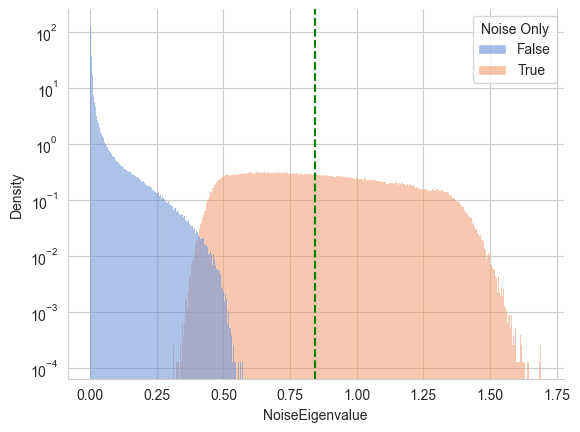
\includegraphics[width=0.5\textwidth]{figures/04_ModelOrderEstimation/noise_eigval_distrib.png}}}
    % \hspace{0.5cm}
    \subfloat[]{{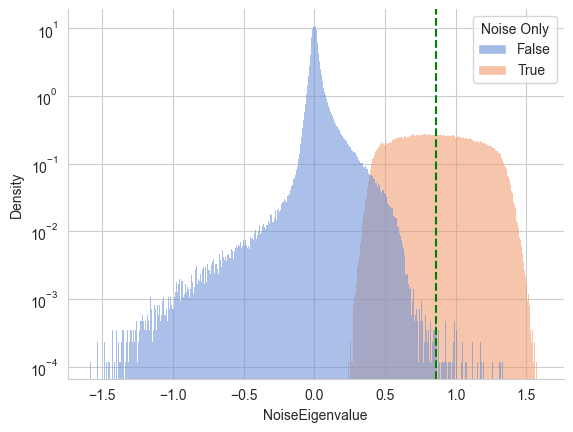
\includegraphics[width=0.5\textwidth]{figures/04_ModelOrderEstimation/noise_eigval_distrib_sub.png}}}
    \caption{Density estimates of noise eigenvalues of the full (a) and sub-sampled (b) covariance matrices, and \( K = 100 \).}
    \label{fig:noise_eigval_distrib}
\end{figure}

\autoref{fig:noise_eigval_distrib} depicts the density estimates of noise eigenvalues for both full and sub-sampled
covariance matrices, given a set number of snapshots \( K = 100 \).
The dataset was generated with a specified noise level of \( P_\eta = -120 \, \si{\deci\bel}_{(\si{\micro\volt})} \),
equating to a noise variance of \( \sigma^2_\eta = 1 \si{\micro\volt\squared} \). \\
The theoretical expectation for the distribution of the noise eigenvalues is given by~\autoref{eq:eigval_superimposed} and
assumes normally distributed noise eigenvalues around \( \sigma^2_\eta \).\\
In the noise-only case, where no signals are present (\( N = 0 \)), the orange distributions indeed aligns with this prediction.
However, the blue distribution, representing scenarios with one to five signals (\( N \in \{1, \ldots, 5\} \)), deviates
from this pattern.

\begin{figure}[H]
    \centering
    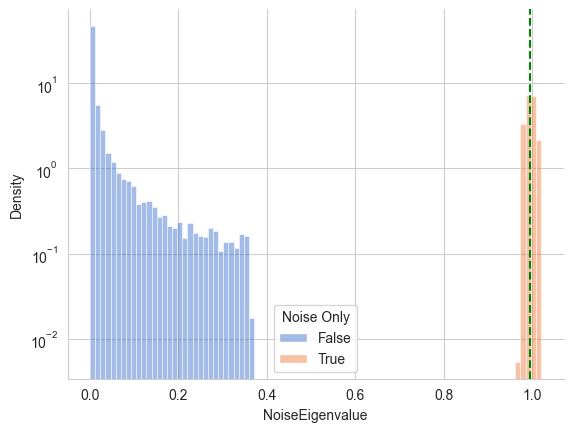
\includegraphics[width=0.45\textwidth]{figures/04_ModelOrderEstimation/noise_eigval_distrib_100k.png}
    \caption{Distribution of noise eigenvalues for \( K = 1e5 \).}
    \label{fig:noise_eigval_distrib_100k}
\end{figure}
Notably, with an increased snapshot count (\( K = 1e5 \)), depicted in \autoref{fig:noise_eigval_distrib_100k}, the
central tendency of the noise eigenvalues for \( N = 0 \) shifts closer to \( \sigma^2_\eta \) which is
in line with expectations. However, the separation between the two clusters—one corresponding to the noise-only case and
the other where signals are present— cannot be explained by the theoretical expectations. \\
Considering that this behavior is consistent across independent simulation environments, it is reasonable to assume that
this bifurcation cannot be explained by a simple ``bug'' in either simulation environment.\\

\subsubsection{Influence of the Model Order}
The emergence of negative eigenvalues within sub-sampled covariance matrices exhibits a strong correlation with the
true model order \( N \). As the complexity of the underlying model increases, the fidelity of the estimated sub-sampled covariance matrix
\( \Csub \) to the true covariance matrix \( \bfm{C}_x \) deteriorates \(\sim\: N \uparrow\; \rightarrow \; \mathcal{L}(\bfm{C}_x, \Csub) \uparrow \).\\
This deterioration is manifested through an increased likelihood of \( \Csub \) losing its positive semi-definiteness.

\begin{figure}[H]
    \centering
    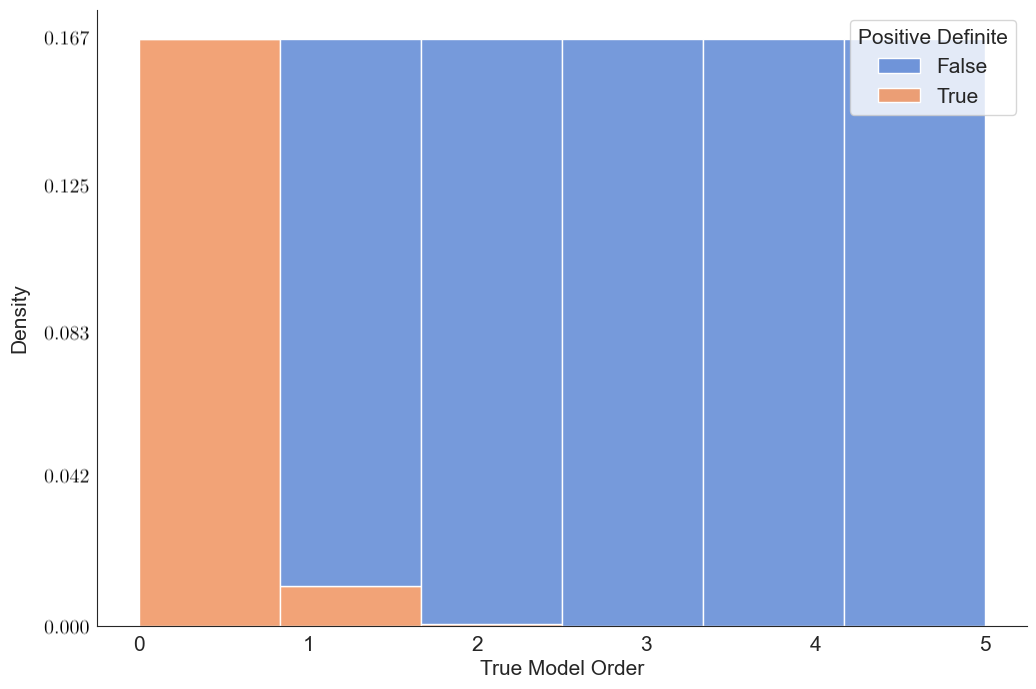
\includegraphics[width=0.45\textwidth]{figures/04_ModelOrderEstimation/eigval_PD_N.png}
    \caption{Illustration of the declining positive definiteness with increasing model order \( N \).}
    \label{fig:eigval_pd_n}
\end{figure}

\autoref{fig:eigval_pd_n}%
\footnote{The data depicted in \autoref{fig:eigval_pd_n} originates from the dataset \( \DMain_{(\text{test})} \), which is discussed in~\autoref{ch:dataset_generation}.}
demonstrates that, at \( K = 100 \), a considerable majority of samples with \( N > 0 \)
experience a loss of positive semi-definiteness in the sub-sampled covariance matrix. \\
Nonetheless, as detailed in~\autoref{ch:evaluation_results}, obtaining reliable model order estimates remains feasible
using the \gls{aic} and \gls{mdl} criteria for most samples where the model order \( N \) is less than the number of RF chains (\( N < L = 3 \)). Furthermore, both the \gls{eft} and deep learning models have been shown to provide accurate model order estimates for \( N \leq 3 \). Empirical evidence indicates that
the eigenvalues retain the ability to encapsulate essential information, enabling accurate predictions of \( N \) even when \( N > 3 \).


\begin{figure}[H]
    \centering
    \subfloat[]{{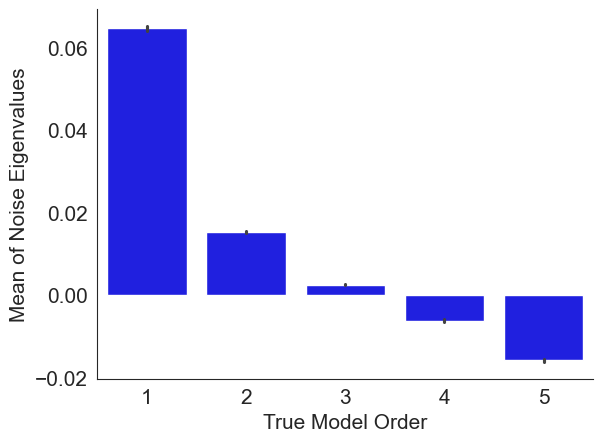
\includegraphics[width=0.37\textwidth]{
        figures/04_ModelOrderEstimation/noise_mean_N.png
    }}}
    \subfloat[]{{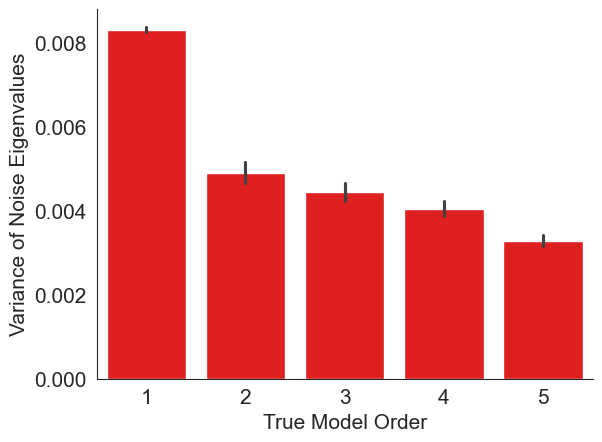
\includegraphics[width=0.37\textwidth]{
        figures/04_ModelOrderEstimation/noise_var_N.png
        }}}
    \caption{
        Mean (a) and variance (b) of the noise eigenvalues for varying model orders \( N \).
    }
    \label{fig:noise_eigval_mean_var_vs_N}
\end{figure}

\autoref{fig:noise_eigval_mean_var_vs_N} illustrates the mean and variance of the noise eigenvalues for varying model orders \( N \).
For sake of interpretability of the linearly scaled y-axis, the mean of the noise eigenvalues for \( N = 0 \) has been omitted from
the plot. \\
The clear correlation between the model order \( N \) and the mean and variance of the noise eigenvalues, can be interpreted
as evidence that the sought-after information about the model order is still encoded within the eigenstructure of the sub-sampled
covariance matrix. Another positive observation is that the \( 95\% \) confidence intervals of mean, as well as the variances
are approximately an order of magnitude smaller than the mean values.

\subsubsection{Influence of the SNR and Number of Snapshots}

Considering that positive definiteness of the covariance matrix seems only to occur for \( N \leq 1 \) for \( K = 100 \),
an evaluation of the relationship between the \gls{sir} and the probability of encountering negative eigenvalues
does not seem to be particularly insightful.\\
However, since both the \( \SNRmin \) and \( \SNRmax \) can already be defined for \( N = 1 \), it appears worthwhile to
investigate the influence of the \gls{snr} on the occurrence of negative eigenvalues.

\begin{figure}[H]
    \centering
    \subfloat[]{{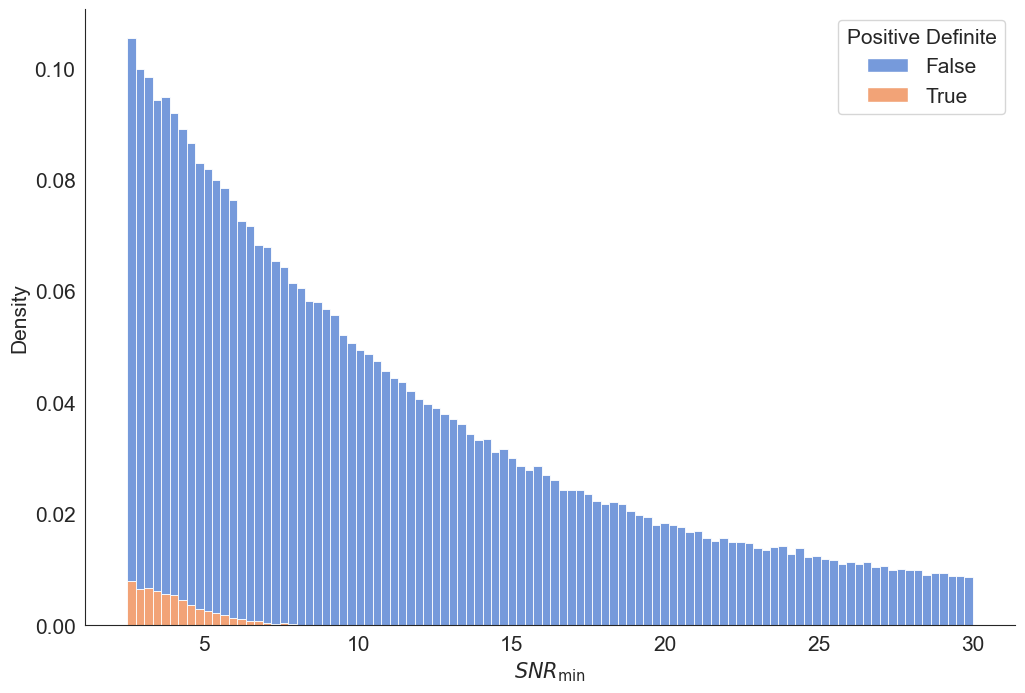
\includegraphics[width=0.33\textwidth]{figures/04_ModelOrderEstimation/snr_hist/min_PD.png}}}
    % \hspace{0.5cm}
    \subfloat[]{{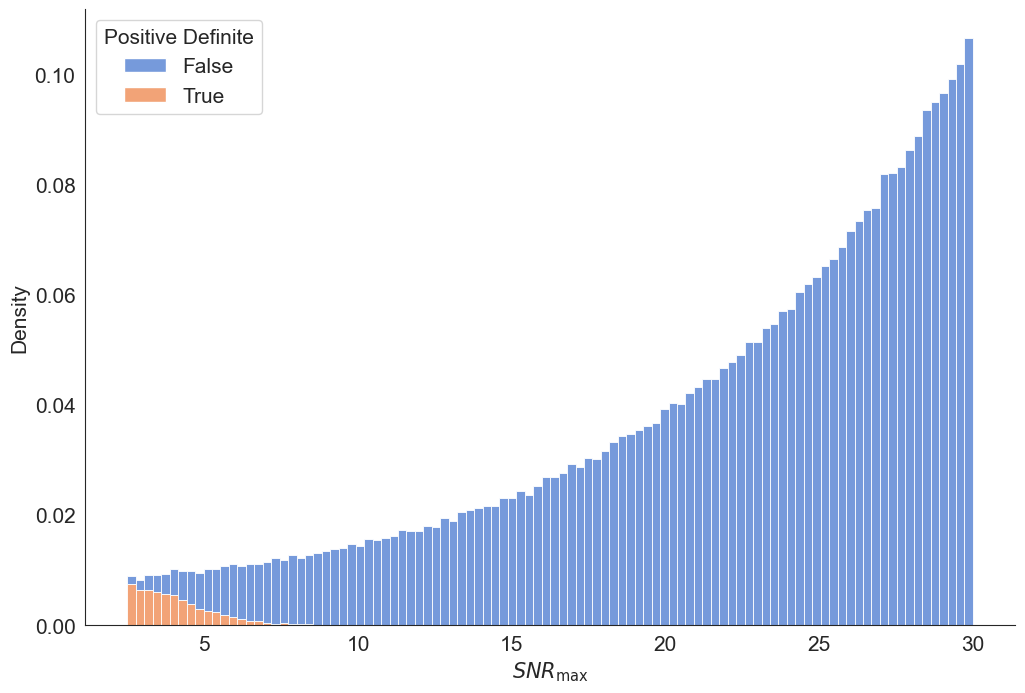
\includegraphics[width=0.33\textwidth]{figures/04_ModelOrderEstimation/snr_hist/max_PD.png}}}
    \caption{Histograms of the \( \SNRmin \) (a), \( \SNRmax \) (b), differentiated w.r.t.\ the positive definiteness.}
    \label{fig:snr_sir_hist}
\end{figure}

\autoref{fig:snr_sir_hist} illustrates the histograms of the \( \SNRmin \) and \( \SNRmax \) values, differentiated with
respect to the positive definiteness of the sub-sampled covariance matrix. \\
As elucidated in the previous chapter, the \gls{pdf} of the \gls{snr} is expected to be a uniform distribution. Utilizing
this knowledge to interpret the histograms, it is evident, that \( \Csub \) quickly loses its positive semi-definiteness
for increasing \( \SNRmin \) and \( \SNRmax \) values.\\


Further insights into the occurrence of negative eigenvalues can be gained by investigating the influence of the number of
snapshots \( K \). Our theoretical expectation is that the sub-sampled covariance matrix should converge asymptotically to the true covariance
matrix -- \( \Csub \rightarrow \bfm{C}_x \) as \( K \rightarrow \infty \). \\
We will therefore investigate the probability of encountering negative eigenvalues for varying numbers of snapshots \( K \)
on the dataset \( \DKvar \) for \( 1 \leq K \leq 1000 \). Subsequently, we will include the \gls{snr} into this evaluation
and present a two-dimensional analysis of the occurrence of negative eigenvalues.

\begin{figure}[H]
    \centering
    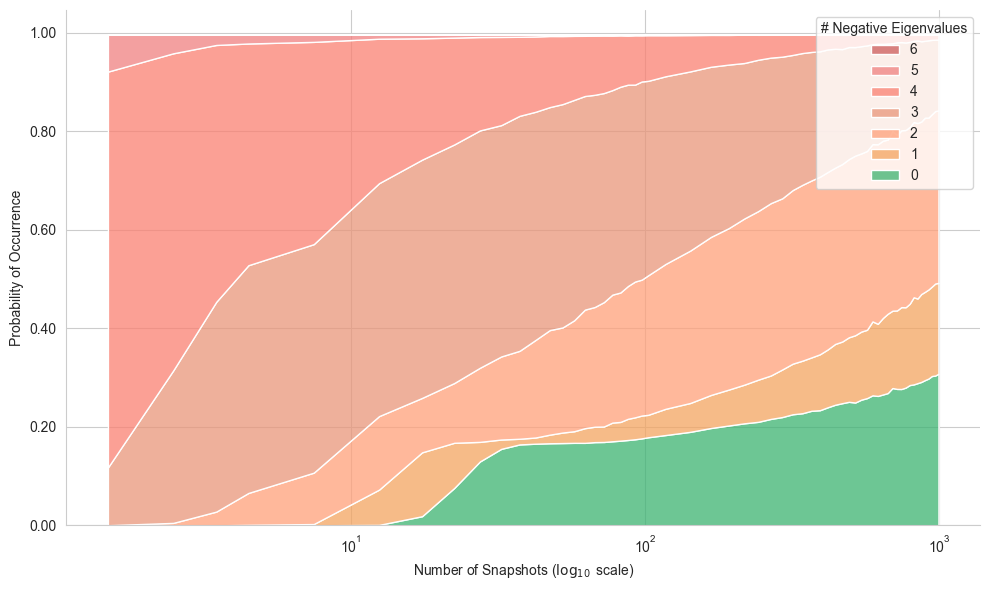
\includegraphics[width=0.8\textwidth]{figures/04_ModelOrderEstimation/num_neg_eigvals_vs_K.png}
    \caption{Probability of encountering \( \ell_{\textit{neg}} \) negative eigenvalues for varying numbers of snapshots \( K \).}
    \label{fig:num_neg_eigvals_vs_K}
\end{figure}

\autoref{fig:num_neg_eigvals_vs_K} illustrates that the likelihood of \( \Csub \) being positive semi-definite asymptotically
increases with \( K \), aligning with theoretical insights presented in~\cite{meyer}.
According to the observations, depicted in~\autoref{fig:eigval_pd_n}, the probability of encountering negative eigenvalues
at \( K = 100 \) should be approximately
\[
    \Pr(\ell_{\textit{neg}} > 0|K=100) = 1 - \Pr(\ell_{\textit{neg}} = 0| K=100) \approx  1 - (0.1\overline{6} + 0.01) = 0.82\overline{3}.
\]

Given the close agreement between both%
\footnote{\autoref{fig:eigval_pd_n} being observed on \( \DMain_{(\text{test})} \) and \autoref{fig:num_neg_eigvals_vs_K} on \( \DKvar \) for \(K = 100\).}
observed probabilities, we are poised to continue with the two-dimensional analysis.



\begin{figure}[H]
    \centering
    \subfloat[]{{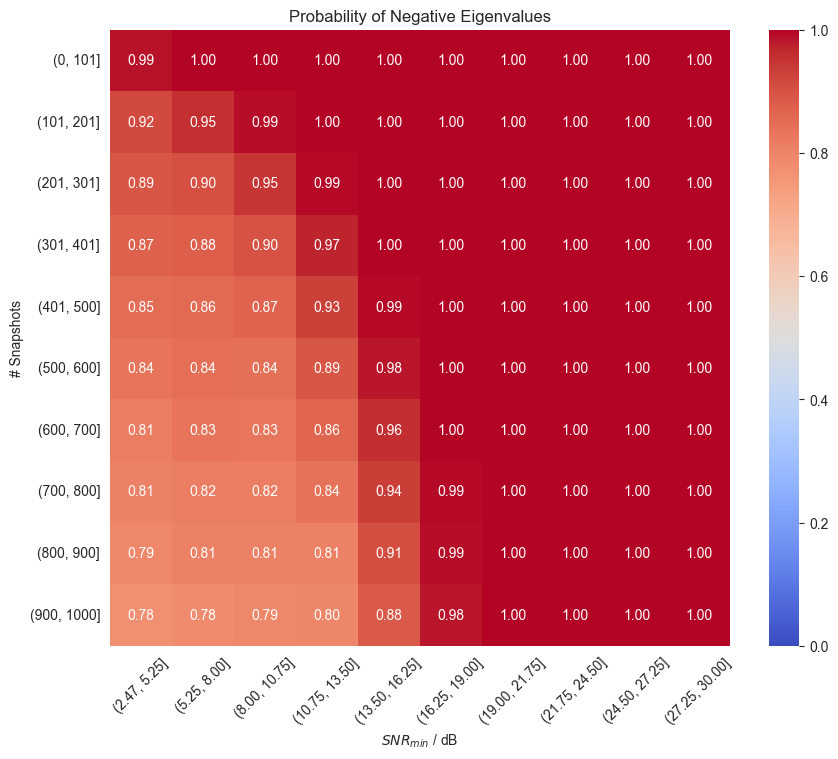
\includegraphics[width=0.45\textwidth]{figures/04_ModelOrderEstimation/snr_min.png}}}
    % \hspace{0.5cm}
    \subfloat[]{{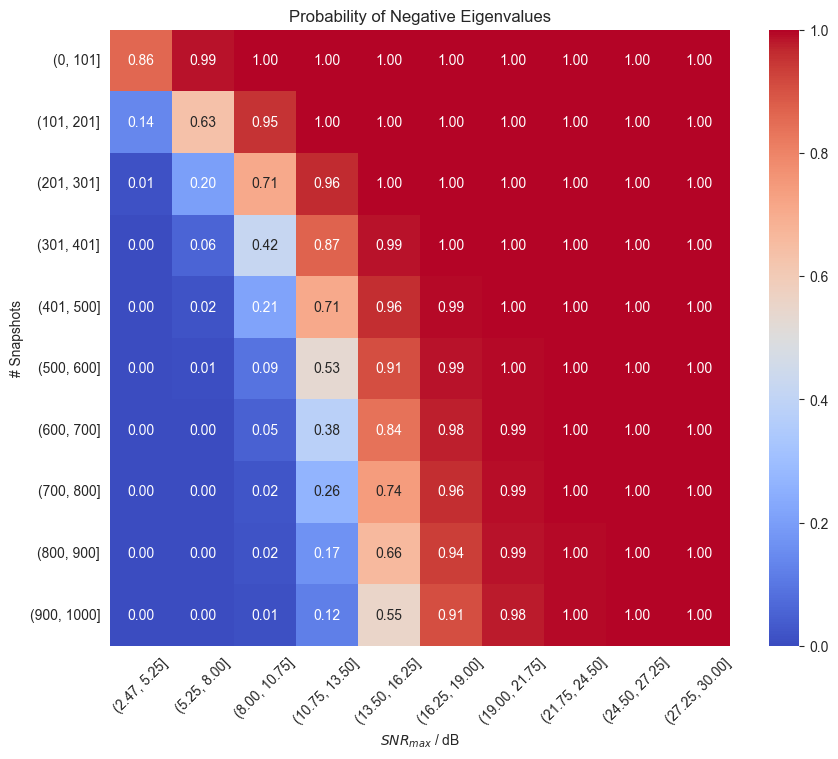
\includegraphics[width=0.45\textwidth]{figures/04_ModelOrderEstimation/snr_max.png}}}
    \caption{Probabilities of negative eigenvalues for the minimum (a) and maximum (b) \gls{snr}, for a varying number
    of snapshots.}
    \label{fig:snr_num_snapshots_pd}
\end{figure}

\autoref{fig:snr_num_snapshots_pd} shows that high \( \SNRmin \) and \( \SNRmax \) values strongly correlated with a
higher probability of negative eigenvalues. Whereas the \( \Pr(\ell_{\textit{neg}} > 0) \) seems to be mostly dependent
on \( N \) for \( K = 100 \), it is evident that other even hg


\subsubsection{Handling Negative Eigenvalues}
To still be able to use the beforementioned algorithmic methods, the eigenvalues need to be transformed so that the resulting
vector \( \bfL \) only contains non-negative values.
Since the \gls{aic}, \gls{mdl}, and \gls{eft} cannot cope with non-positive eigenvalues, they had to be inferred from transformed
eigenvalues \( \widetilde{\bfL} \) whose positivity was ensured according to~\autoref{eq:pos_eigvals}.

\begin{align}
    \widetilde{\bfm{\lambda}} &=
    \begin{cases}
      \bfm{\lambda} + \lambda_M + \epsilon_{\text{eft}} & \text{if } \lambda_M \leq \epsilon_{\text{eft}} \text{ for \gls{eft}}, \quad \epsilon_{\text{eft}} = \num{1e-6} \\
      \bfm{\lambda} + \lambda_M + \epsilon_{\text{IC}} & \text{if } \lambda_M \leq \epsilon_{\text{IC}} \text{ for \gls{aic} and \gls{mdl}}, \quad \epsilon_{\text{IC}} = \num{1} \\
      \bfm{\lambda} & \text{otherwise}
    \end{cases}
    \label{eq:pos_eigvals}
\end{align}

The additional offset term \( \epsilon_{\text{IC}} \) was introduced to ensure that \( \widetilde{\bfm{\lambda}}_{\text{IC}} \)
does not contain any values close to zero, which would result in most criteria values \( \bfm{\mathrm{AIC}}[n] \)  and \( \bfm{\mathrm{MDL}}[n] \) diverging to
\( \infty \). Lower values of \( \epsilon_{\text{IC}} \) appear to be correlated with a higher bias. A value of \( \epsilon_{\text{IC}} = 1 \) was chosen,
since \( \sigma^2_{\eta} = 1 \), and therefore the noise eigenvalues \( \bfm{\lambda}_{\eta} \) are expected to cluster around 1.\\
\gls{mdl} exhibited a slightly better performance in terms of bias and variance for eigenvalues \( \widetilde{\bfL} \) being
transformed by
\begin{equation}
    \mathcal{TF} \coloneq \{\| \bullet \| \rightarrow \text{sort}(\bullet) \rightarrow \bullet = \bullet + \epsilon_{\text{IC}}\}, \quad \mathcal{TF} : \bfL \mapsto \widetilde{\bfL}.
\end{equation}
The \gls{eft}, conversely, only requires a small offset to ensure that the eigenvalues are greater than zero. Increasing
the offset reduces the goodness of fit of the \gls{eft}'s predicted eigenvalue profile to the true eigenvalues.

% \section{Factors Influencing \gls{moe}}
% The \gls{moe} methods discussed in this thesis depend on the distribution of eigenvalues. Important factors influencing \gls{moe}
% include the \glsfirst{snr}, \glsfirst{sir}, the array's aperture \( D \), finite-sample effects when \( K < 10M \),
% modeling errors, and the impact of sub-sampling. As the conventional methods used at Rohde \& Schwarz are affected by
% these factors, they will be discussed further at the end of this chapter~\cite{meyer}.\\


% - multipath -> rank deficient -> overfitting -> higher model order: `By partitioning the whole array into sub-
% arrays and averaging of the sub-array received covariance matrices, the equivalent source covariance matrix becomes
% nonsingular. The FBSS scheme is widely-used since it can be regarded as a preprocessing before applying AIC and MDL [9]
% as well as DOA estimation algorithms`'\cite{yang2020}

% ---

% \begin{align}
%     \mathcal{H}_{p+1} &: \lambda_{M-p} \in \bfL_\eta \label{eq:hypothesis_noise} \\
%     \widetilde{\mathcal{H}}_{p+1} &: \lambda_{M-p} \in \bfL_S \label{eq:hypothesis_signal}
% \end{align}

% Starting with the pair \( (\lambda_{M-1}, \hat{\lambda}_{M-1}) \), the relative distance between each of the
% theoretical noise eigenvalues and their corresponding observed eigenvalue is computed. This difference is then assessed
% against a predefined threshold value \( \tau_n \), which scales with the eigenvalue index. The condition for
% determining the hypothesis to accept is as follows:

% \begin{equation*}
%     \lambda \in \left\{
%         \begin{array}{ll}
%             \bfL_{\eta}, & \text{if } \left|\frac{\lambda_{M-p} - \hat{\lambda}_{M-p}}{\hat{\lambda}_{M-p}}\right| = \epsilon_n \leq \tau_n, \\
%             \bfL_{S}, & \text{otherwise}.
%         \end{array}
%     \right.
% \end{equation*}